\documentclass[]{article}

% Use utf-8 encoding for foreign characters
%\usepackage[latin1]{inputenc}


% Setup for fullpage use
\usepackage{fullpage}
% Uncomment some of the following if you use the features
%
% Running Headers and footers
%\usepackage{fancyhdr}

% Multipart figures ´¡009753º
% More symbols
%\usepackage{amsmath}\emph{}
%\usepackage{amssymb}
%\usepackage{latexsym}

% Surround parts of graphics with box
\usepackage{boxedminipage}

% Package for including code in the document
\usepackage{listings}

% Package for subfigure
\usepackage{graphicx}


% If you want to generate a toc for each chapter (use with book)
\usepackage{minitoc}

% This is now the recommended way for checking for PDFLaTeX:
\usepackage{ifpdf}
%\newif\ifpdf
%\ifx\pdfoutput\undefined
%\pdffalse % we are not running PDFLaTeX
%\else
%\pdfoutput=1 % we are running PDFLaTeX
%\pdftrue
%\  XCM CNXKJBWQGFUHREPUYT485¨94-32¨1fi
\usepackage[all,light]{draftcopy}
%\draftcopyName{PROBABILIDAD II}{5}


\usepackage{amsmath}
\usepackage{amsfonts}
\usepackage{bm}
\usepackage{layout}
\usepackage{fancyhdr}
\usepackage{subcaption}
\pagestyle{fancy}
%\fancyhf{}
\newlength\FHoffset
\setlength\FHoffset{0.1cm}
%\addtolength\headwidth{2\FHoffset}
\fancyheadoffset{\FHoffset}
%\ifpdf
%\usepackage[pdftex]{graphicx}
%\else
%\usepackage{graphicx}
%\fi
\usepackage[top=2cm,bottom=2cm,left = 1cm, right = 1cm,headsep=1.5cm]{geometry}
\usepackage{hyperref}
\newcommand{\R}{\mbox{$I\!\!R$}}
\usepackage{cleveref}

\begin{document}

\lhead{\textsf{UCSC - Fall 2016} \\{AMS 374}}
\chead{\Large{General Linear Model}}
\rhead{\textsf{Student:} \\{Rui Meng}}
\renewcommand{\headrulewidth}{0.4pt}
\renewcommand{\footrulewidth}{0.4pt}


\begin{center}
\section*{\underline{Homework 3}}
\end{center}

\begin{enumerate}  \Large{
		\item (Ex 1)
		The table below reports results from a toxicological experiment, including the number of beetles killed $(y_i)$ after $5$ hours exposure to gaseous carbon disulphide at various concentrations. Concentration (log dose, $x_i$) is given on the $\log_{10}$ scale.\\
		\begin{table}[ht]
			\centering
			\begin{tabular}{ccc}
				\hline
				Log Dose, $x_i$ & Number of beetles, $m_i$ & Number killed, $y_i$ \\
				\hline
				1.6907 & 59 & 6 \\
				1.7242 & 60 & 13 \\
				1.7552 & 62 & 18 \\
				1.7842 & 56 & 28 \\
				1.8113 & 63 & 52 \\
				1.8369 & 59 & 53 \\
				1.8610 & 62 & 61 \\
				1.8839 & 60 & 60 \\
				\hline
			\end{tabular}
		\end{table}
        Consider a binomial response distribution, and assume that the $y_i$ are independent realizations from $\mathrm{Bin}(m_i,\pi_i)$, $i = 1,\ldots,n$. The objective is to study the effect of the choice of link function $g(\cdot)$, where $\pi_i = g^{-1}(\eta_i) = g^{-1}(\beta_1 + \beta_2x_i)$.\\
        \begin{itemize}
        	\item[(a)] Using R, fit binomial GLMs for these data corresponding to 3 link functions, logit, probit an complementary log-log. Perform residual analysis for each model, using the deviance residuals. Obtain fitted values, $\hat{\pi}_i$, under each model and compare with observed proportions, $y_i/m_i$. Obtain the estimated dose-response curve under each model by evaluating $\hat{\pi}(x) = g^{-1}(\hat{\beta}_1 + \hat{\beta}_2x)$ over a grid of values $x$ for log dose in the interval $(1.65,1.9)$. Plot these curves and compare with the scatter plot of the observed $x_i$ plotted against the observed proportions. Based on all the results above, discuss the fit of the different models.
        	\item[(b)] One of the more general (parametric) link function for binomial GLMs that has been suggested in the literature is defined through
        	\begin{equation}
        	g_\alpha^{-1}(\eta_i) = \frac{\exp(\alpha\eta_i)}{\{1+\exp(\eta_i)\}^\alpha} \mathrm{ for } \alpha>0.
        	\label{1}
        	\end{equation}
        	Note that the logit link arises as a special case of \ref{1}, where $\alpha = 1$. Discuss the effect of the additional model parameter $\alpha$, in particular, for values $0<\alpha<1$ and $\alpha>1$. Provide the expression for the log-likelihood for $\beta_1$, $\beta_2$ and $\alpha$ under the link in \ref{1}, and discuss the complications that arise for maximum likelihood estimation under this more general model compared with the logit GLM. (You do not need to fit the model, estimates are given below.)
        	\item[(c)] The MLEs under model with link given in \ref{1} are $\hat{\beta}_1 = -113.625$, $\hat{\beta}_2 = 62.5$ and $\hat{\alpha} = 0.279$. (The MLEs can be obtained using the Newton-Raphson method.) Using these estimates, obtain the fitted values $\hat{\pi}_i$ and the estimated dose-response curve under the link \ref{1}. Compare with the corresponding results under the 3 models in (a). Obtain the deviance residuals from the model with link \ref{1} and analyze them graphically.
        	\item Compute the AIC and BIC for the 4 models considered above to compare them.
        \end{itemize}
        \item[Sol 1]
        \begin{itemize}
        	\item[(a)] 
        	The residual analysis for three models with logit, probit and complementary log-log link functions is summarized as following: Their mean function are $g^{-1}(\bm{X}\bm{\beta}) = \frac{1}{1+\exp(-\bm{X}\bm{\beta})}$, $g^{-1}(\bm{X}\bm{\beta}) = \Phi(\bm{X}\bm{\beta})$ and $g^{-1}(\bm{X}\bm{\beta}) = 1 - \exp[-\exp(\bm{X}\bm{\beta})]$.\\
        	First, the deviance residuals for three models are shown in Table~\ref{0}.\par
        	\begin{table}[ht!]
        		\centering
        		\caption{Deviance residuals for four models: Model 1 refers to logit link; Model 2 refers to probit link; Model 3 refers to complementary log-log link, Model 4 refers to general link function}
        		\begin{tabular}{c|c|c|c|c|c|c|c|c}
        			\hline
        			$\hat{r^D}_{\mathrm{Model 1}}$ & 1.28 & 1.06 & -1.20 & -1.59 &  0.61  & -0.13 & 1.25  & 1.59 \\
        			\hline
        			$\hat{r^D}_{\mathrm{Model 2}}$ & 1.34 & 0.75  & -1.46  & -1.57 &  0.75 &-0.14 & 1.00 & 1.25 \\
        			\hline
        			$\hat{r^D}_{\mathrm{Model 3}}$ & 0.18 & 0.56 & -0.80 & -0.63 & 1.29 &-0.52& -0.12 & 0.32  \\
        			\hline
        			$\hat{r^D}_{\mathrm{Model 4}}$ & -0.17 & 0.42& -0.72& -0.56 & 1.03 &-0.84&  0.12 & 0.73    \\
        			\hline
        		\end{tabular}
        		\label{0}
        	\end{table}
        	Second, the comparison between observed proportions and fitted values for different models are shown in the Table~\ref{cmp}.\par
        	\begin{table}[ht!]
        		\centering
        		\caption{Observed proportions and fitted values for four models: Model 1 refers to logit link; Model 2 refers to probit link; Model 3 refers to complementary log-log link, Model 4 refers to general link function}
        		\begin{tabular}{c|c|c|c|c|c|c|c|c}
        			\hline
        			$y_i/m_i$ & 0.10 & 0.22 & 0.29 & 0.50 & 0.83 & 0.90 & 0.98 & 1.00 \\
        		    \hline
        		    $\hat{\pi}_{\mathrm{Model 1}}$ & 0.06 & 0.16 & 0.36 & 0.61 & 0.80 & 0.90 & 0.96 & 0.98\\
        		    \hline
        		    $\hat{\pi}_{\mathrm{Model 2}}$ & 0.06 & 0.18 & 0.38 & 0.60 & 0.79 & 0.90 & 0.96 & 0.99\\
        		    \hline
        		    $\hat{\pi}_{\mathrm{Model 3}}$ & 0.09 & 0.19 & 0.34 & 0.54 & 0.76 & 0.92 & 0.99 & 1.00 \\
        		    \hline
        		    $\hat{\pi}_{\mathrm{Model 4}}$ & 0.11 & 0.19 & 0.33 & 0.54 & 0.77 & 0.93 & 0.98 & 1.00\\
        		    \hline
        		\end{tabular}
        		\label{cmp}
        	\end{table}
            Third, estimated dose-response curves under each model are estimated in the interval $(1.65, 1.9)$ and plotted with the observed $x_i$ against the observed proportion in Figure~\ref{2}. Those figures show the model with complementary log-log link is better than other two because the estimated curve is closer to observed points.
            \begin{figure}[ht!]
            	\centering
            	\begin{subfigure}[b]{0.3\textwidth}
            		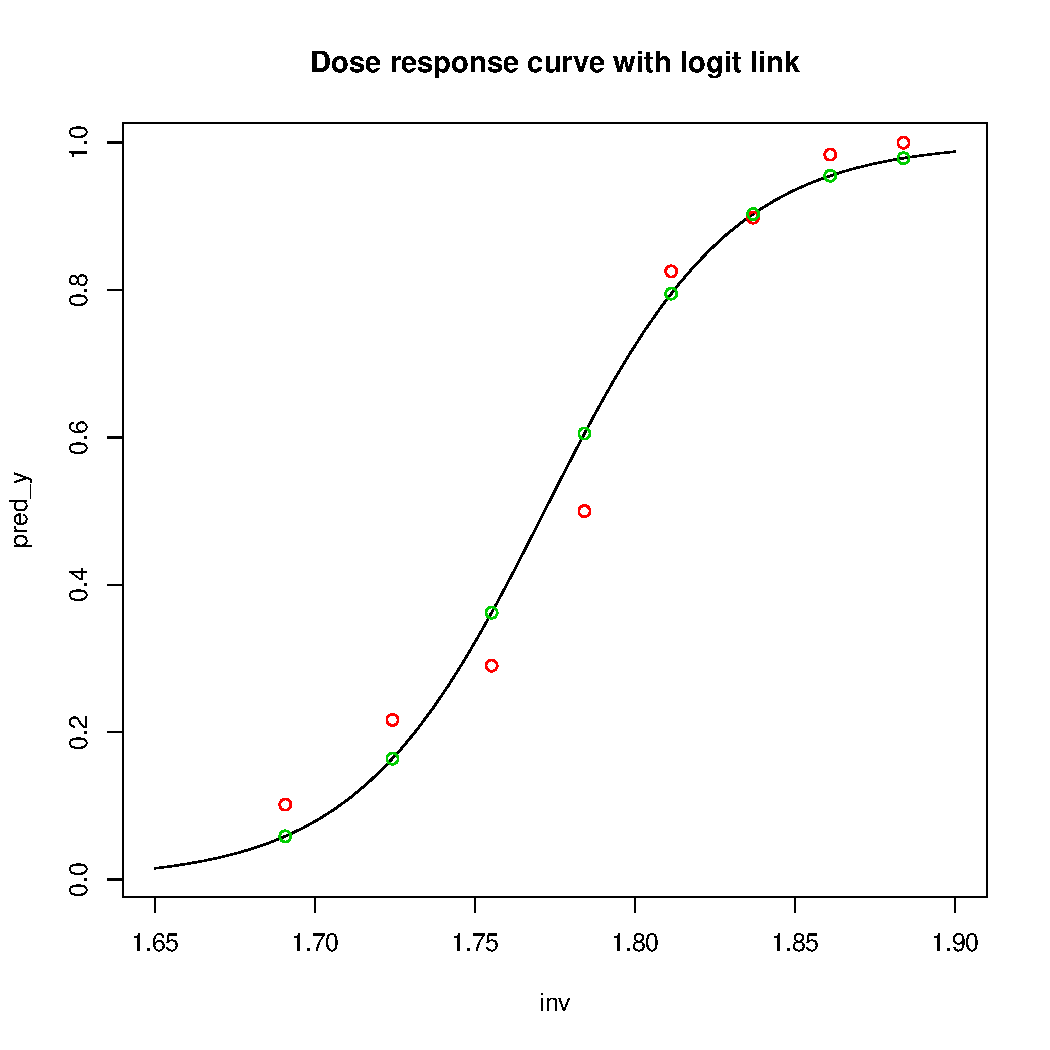
\includegraphics[width = \textwidth]{pic/HW3_1/a1.pdf}
            	\end{subfigure}
            	\begin{subfigure}[b]{0.3\textwidth}
            		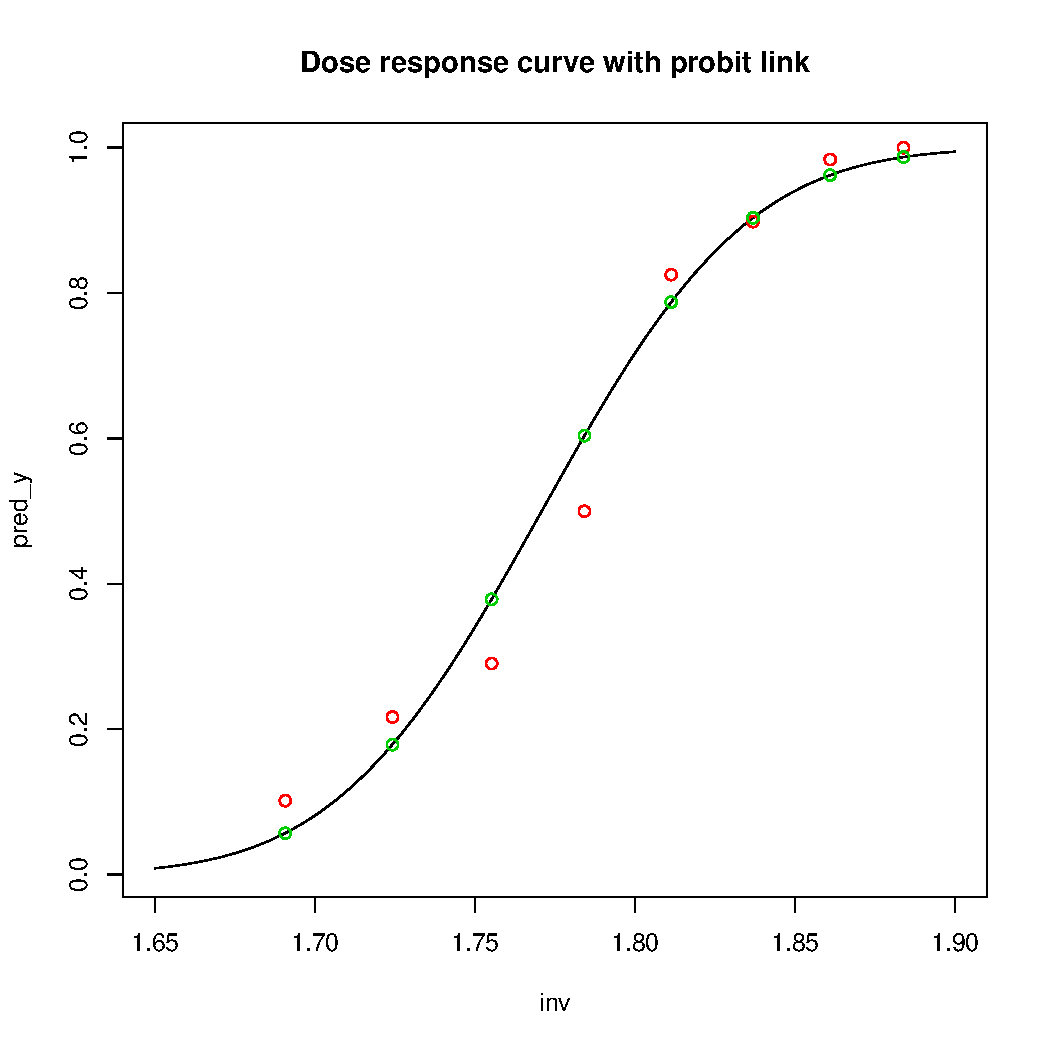
\includegraphics[width = \textwidth]{pic/HW3_1/a2.pdf}
            	\end{subfigure}
            	\begin{subfigure}[b]{0.3\textwidth}
            		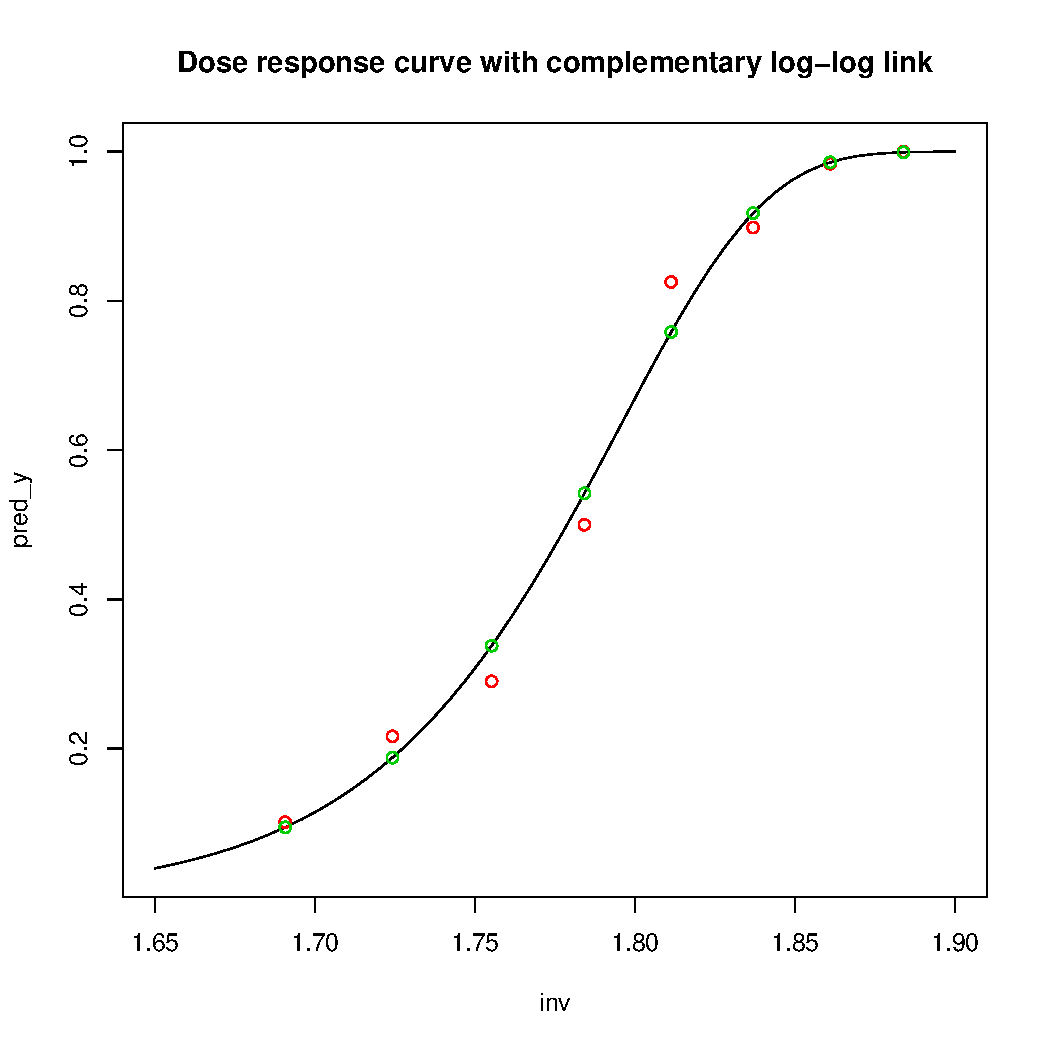
\includegraphics[width = \textwidth]{pic/HW3_1/a3.pdf}
            	\end{subfigure}
            	\caption{Three estimated dose-response curves compared with the observed $x_i$ plotted against the observed proportions}
            	\label{2}
            \end{figure}
        	
        	\item[(b)]
        	Figure~\ref{3} shows that as $\alpha$ increases the mean function is going to become a step function with the jump point $0$, which suggests that the MLE is more likely close to $0$ or $1$.
        	\begin{figure}[ht!]
        		\centering
        		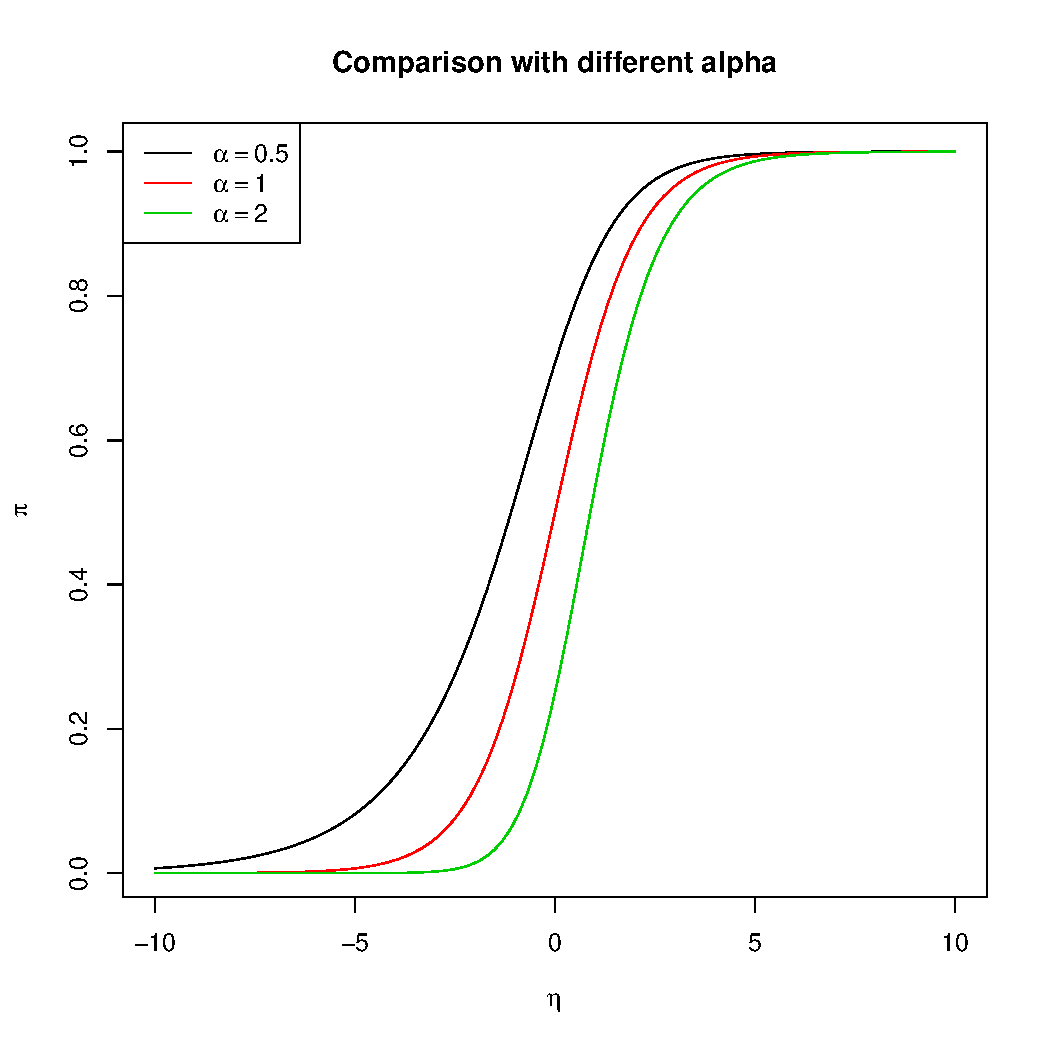
\includegraphics[width = 0.5\textwidth]{pic/HW3_1/b.pdf}
        		\caption{The link function with different $\alpha$}
        		\label{3}
        	\end{figure}
        	And the log-likelihood is derived as follows
        	\begin{eqnarray}
        	\ell(\bm{\beta}, \alpha|\bm{y}) & = & \sum_{i = 1}^{n}(y_i\log(\frac{\pi_i}{1-\pi_i}) + m_i\log(1-\pi_i) + \log\begin{bmatrix}
        	m_i\\ y_i
        	\end{bmatrix}) \\
        	& = & \sum_{i = 1}^{n} (y_i\log(\frac{\exp(\alpha\bm X\bm\beta)}{(1+\exp(\bm X\bm{\beta}))^\alpha - \exp^{\alpha\bm{X}\bm\beta}}) +\\
        	& & m_i\log(\frac{(1+\exp(\bm X\bm{\beta}))^\alpha - \exp^{\alpha\bm{X}\bm\beta}}{(1+\exp(\bm X\bm{\beta}))^\alpha}) + \log\begin{bmatrix}
        	m_i \\ y_i
        	\end{bmatrix}  )\,.
        	\end{eqnarray}
        	Maximizing $\ell(\bm{\beta}, \alpha|\bm{y})$ is difficult, because of the complexity of $(1+\exp(\bm X\bm{\beta}))^\alpha - \exp^{\alpha\bm{X}\bm\beta}$. Compared with the logit link function in which $\alpha = 1$, the complexity can be reduced by $(1+\exp(\bm X\bm{\beta}))^\alpha - \exp^{\alpha\bm{X}\bm\beta} = 1$.
        	\item[(c)] 
        	The fitted values are shown in Table~\ref{1} and the estimated dose-response curve are shown in Figure~\ref{4}.
        	\begin{figure}[h!]
        	    \centering
        	    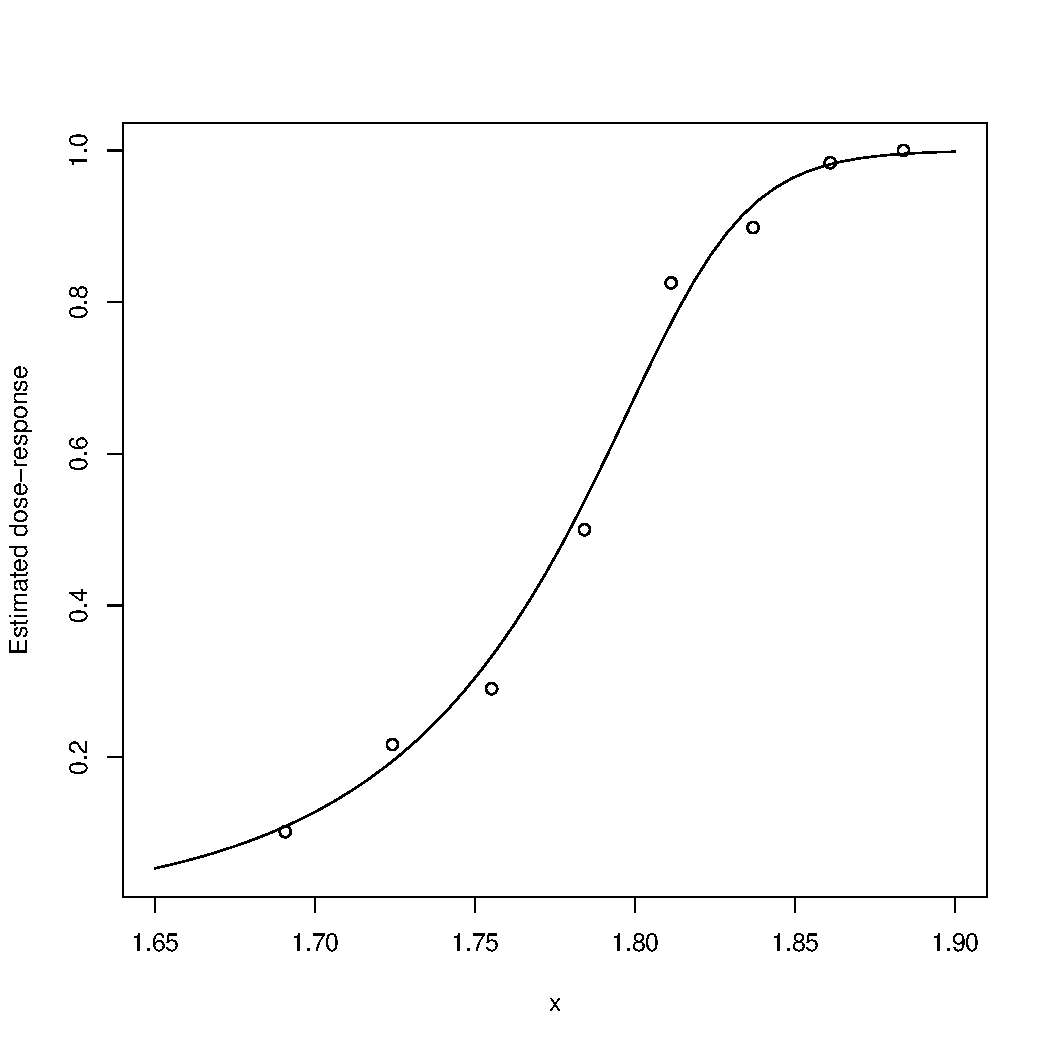
\includegraphics[width = 0.5\textwidth]{pic/HW3_1/c.pdf}
        	    \caption{The dose-response curve with general link function}
        	    \label{4}
        	\end{figure}
        	From the deviance residuals, overall the deviance residuals are closer to 0 compared with the previous models. Also, the observed points are very close to the estimated curve, which illustrates the model with this general link function performs well.
        	
        	\item[(d)] The AIC and BIC are shown in Table~\ref{5}.
        	\begin{table}[h!]
        		\centering
        		\caption{AIC and BIC for four different models}
        		\begin{tabular}{c|c|c}
        			\hline
        			Model & AIC & BIC \\
        			\hline
        			Model 1 & 41.43 & 41.59 \\
        			\hline
        			Model 2 & 40.32 & 40.47 \\
        			\hline
        			Model 3 & 33.64 & 33.80 \\
        			\hline
        			Model 4 & 35.55 & 35.78 \\
        			\hline
        		\end{tabular}
        		\label{5}
        	\end{table}
        	Table~\ref{5} shows that considering the complexity of model, Model 3 performs better than others from both AIC and BIC respective.
        \end{itemize}
        
        \item (Ex 2)
        This problem involves Bayesian analysis of the beetle mortality data from the previous problem.
        \begin{itemize}
        	\item[(a)]Consider a Bayesian binomial GLM with a complementary log-log link, i.e., assume that, given $\beta_1$ and $\beta_2$, the $y_i$ are independent from $\mathrm{Bin}(m_i,\pi(x_i)), i = 1,\ldots,8$, where 
        	$$\pi(x) = \pi(x; \beta_1, \beta_2) = 1 - \exp\{-\exp(\beta_1 + \beta_2 x)\}\,.$$
        	Design and implement an MCMC method to sample from the posterior distribution of $(\beta_1,\beta_2)$. Study the effect of the prior for $(\beta_1,\beta_2)$, for example, consider a flat prior as well as (independent) normal priors. Under the flat prior, obtain the posterior distribution for the median lethal dose, $LD_{50}$, that is, the dose level at which the probability of response is $0.5$. Finally, plot point and interval estimates for the dose-response curve $\pi(x)$ (over a grid of values $x$ for log dose).
        	\item[(b)]Next, consider a binomial GLM with a logit link, i.e., now the $y_i$ are assumed independent, given $\beta_1$ and $\beta_2$, from $\mathrm{Bin}(m_i,\pi(x_i)), i = 1,\ldots,8$, where 
        	$$\pi(x) \equiv \pi(x;\beta_1,\beta_2) = \exp(\beta_1 + \beta_2 x)/\{1+\exp(\beta_1 + \beta_2x)\}.$$
        	Working with a flat prior for $(\beta_1, \beta_2)$, obtain MCMC samples from the posterior distributions for $\beta_1$, $\beta_2$, and for $\mathrm{LD}_{50}$, along with point and interval estimates for the dose-response curve $\pi(x)$.
        	\item[(c)] As a third model, consider the binomial GLM with the parametric link given in \ref{1}. Develop an MCMC method to sample from the posterior distribution of $(\beta_1,\beta_2,\alpha)$, and obtain the posterior distribution for $\mathrm{LD}_{50}$, and point and interval estimates for $\pi(x)$.
        	\item[(d)] Use the results from parts (a), (b) and (c) for an empirical comparison of the three Bayesian binomial GLMs for the beetle mortality data. Moreover, perform a residual analysis for each model using the \textit{Bayesian residuals}: $(y_i/m_i) - \pi(x_i;\beta_1,\beta_2)$ for the first two models, and $(y_i/m_i) - \pi(x_i;\beta_1,\beta_2,\alpha)$ for the third. Finally, use the \textit{quadratic loss L measure} for formal comparison of the three models.
        	
        \end{itemize}
        
        \item[Sol 2]
        \begin{itemize}
        	\item[(a)]
        	As for a Bayesian binomial GLM with a complementary log-log link, the posterior distribution of parameters is
        	\begin{eqnarray}
        	P(\beta_1, \beta_2|\bm x, \bm m, \bm y) & \propto & P(\beta_1, \beta_2|\bm x, \bm m)P(\bm y|\bm x, \bm m, \beta_1, \beta_2)\\
        	& = & P(\beta_1, \beta_2)P(\bm y| \bm x, \bm m, \beta_1, \beta_2)\\
        	& = & P(\beta_1, \beta_2)\prod_{i = 1}^{n}\begin{bmatrix}
        	m_i\\y_i
        	\end{bmatrix}\pi(x_i)^{y_i}(1-\pi(x_i))^{m_i-y_i}\\
        	& = & P(\beta_1, \beta_2) \prod_{i = 1}^{n}(1- \exp\{-\exp(\beta_1+\beta_2x_i)\})^{y_i}\\
        	& &(\exp\{-\exp(\beta_1+\beta_2x_i)\})^{m_i-y_i}\,.
        	\end{eqnarray}
            To compare the different prior effects, we take the flat prior and normal prior for instance.
        	%We can use the slice Gibbs sampling to obtain the posterior distribution of $\bm{\beta}$. Since $P(\beta_1, \beta_2|\bm x, \bm m, \bm y)  \propto \pi(\bm{\beta}) h(\bm{\beta})$, where $h(\bm{\beta}) = \prod_{i = 1}^{n} h_i(\bm \beta) = \prod_{i = 1}^{n}\begin{bmatrix}
        	%m_i\\y_i
        	%\end{bmatrix}(1- \exp\{-\exp(\beta_1+\beta_2x_i)\})^{y_i}(\exp\{-\exp(\beta_1+\beta_2x_i)\})^{m_i-y_i}$, we propose 
        	%\begin{equation}
        	%P(\bm \beta, \bm u) \propto \pi(\bm{\beta})\prod_{i =1}^{n}I\{u_i<h_i(\bm{\beta})\}\,.
        	%\end{equation}
        	%Then $P(\bm u|\bm{\beta}) = \frac{P(\bm{\beta},\bm{\mu})}{P(\bm{\beta})} \propto \prod_{i = 1}^{n}I\{u_i<h_i(\bm{\beta})\}$ and $P(\bm\beta|\bm\mu) = \frac{P(\bm{\beta}, \bm{u})}{P(\bm u)} \propto \pi(\bm{\beta})\prod_{i =1}^{n}I\{u_i<h_i(\bm{\beta})\}$.
        	%Using the slice sampling, we can sample from the posterior distribution of $(\beta_1, \beta_2)$. And the posterior distribution of parameters heavily depends on the prior distribution as well as the convergence speed.\\
        	Using Metropolis Hasting algorithm with both flat prior and standard normal prior, we obtain the posterior distributions of $\bm \beta$ by sampling 1000 times and choosing the burn-in $T = 100$. The posterior distributions are shown in Figure~\ref{6}. Those figures show that the posterior distribution depends on the prior distributions heavily.\par
        	\begin{figure}[ht!]
        		\centering
        		\begin{subfigure}{0.45\textwidth}
        			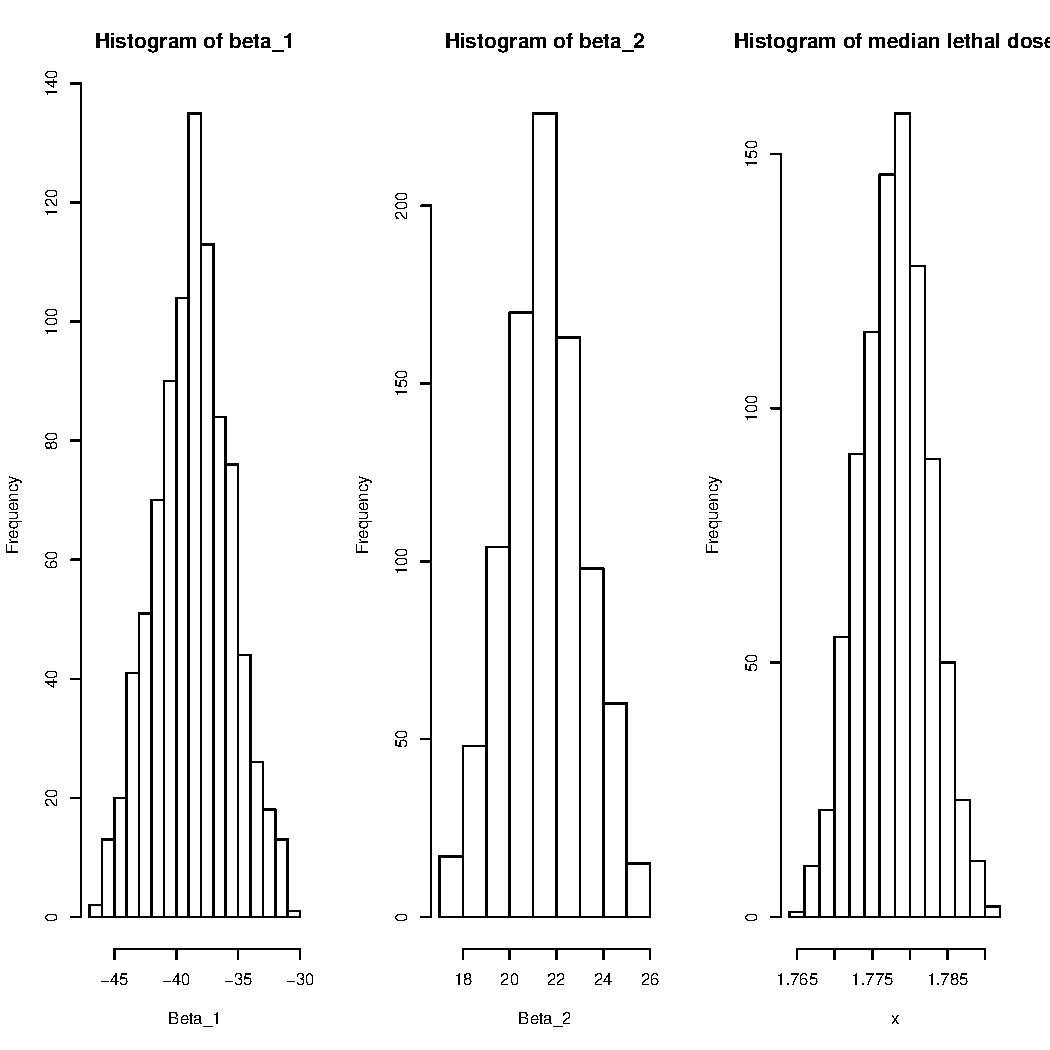
\includegraphics[width = \textwidth]{pic/HW3_2/a1.pdf}
        		\end{subfigure}
        		\begin{subfigure}{0.45\textwidth}
        			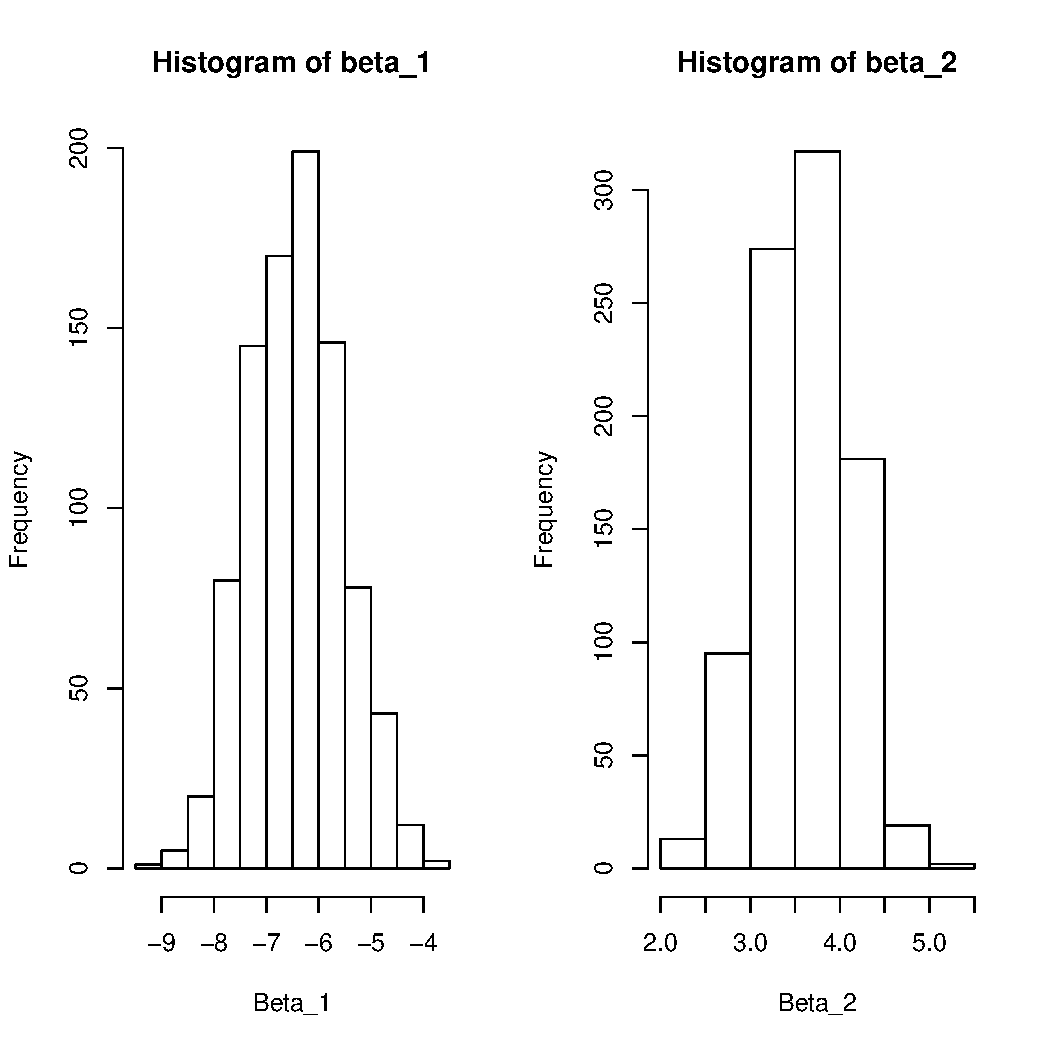
\includegraphics[width = \textwidth]{pic/HW3_2/a2.pdf}
        		\end{subfigure}
        		\caption{The posterior distributions for flat prior and standard normal prior with complementary log-log link function}
        		\label{6}
        	\end{figure}
        	Because $\pi(x) = 1-\exp\{-\exp(\beta_1+\beta_2x)\}$, the median lethal dose is $x_{0.5} = \frac{\log\log 2-\beta_1}{\beta_2}$. Then thanks to calibration inference, the posterior distribution of median lethal dose with flat prior is shown in Figure~\ref{6}. Using 1000 sampled $\bm{\beta}$ with the burn-in $T = 100$, the point and centered $95\%$ confidence interval estimates for the dose-response curve $\pi(x)$ on the grid $[1.65,1.9]$ are plotted in Figure~\ref{7}.
        	\begin{figure}[ht!]
        		\centering
        		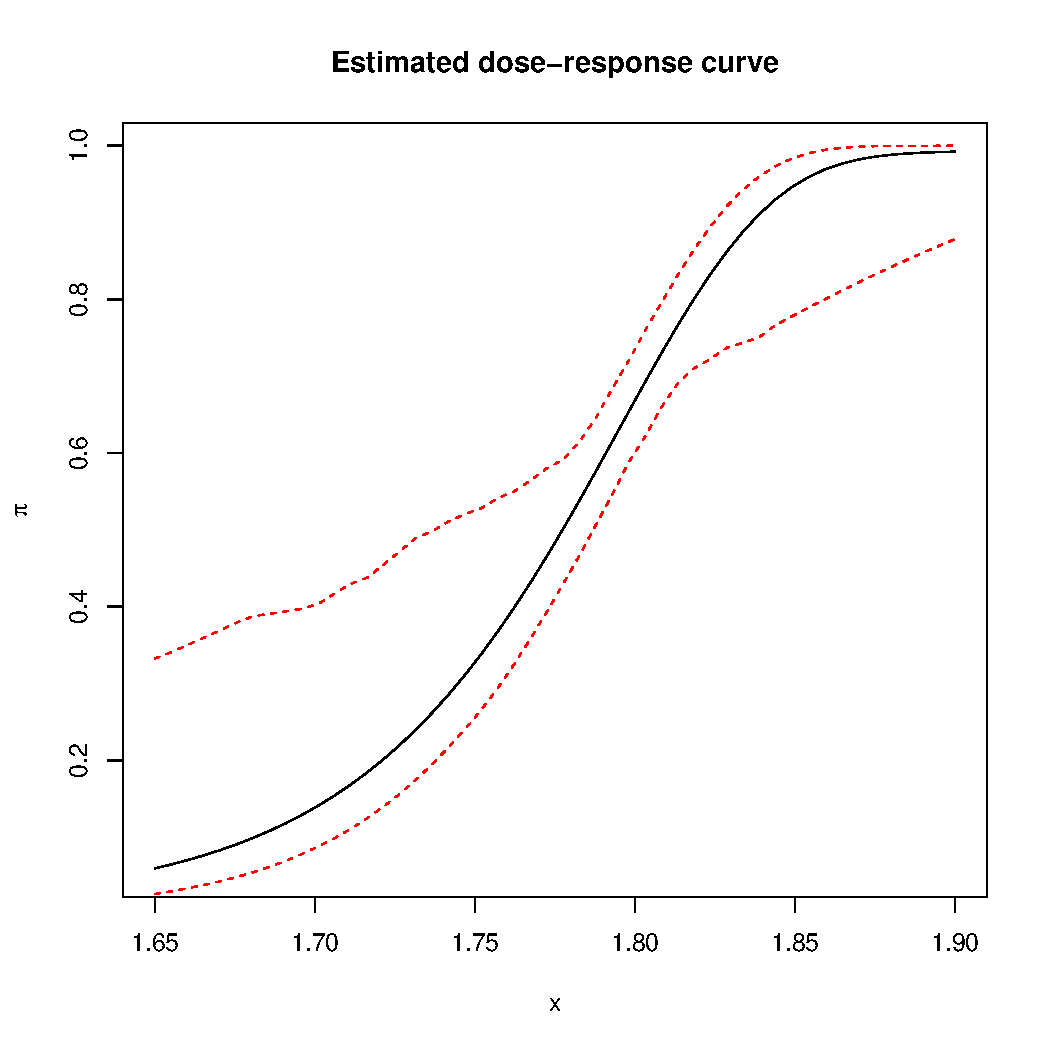
\includegraphics[width = 0.5\textwidth]{pic/HW3_2/a3.pdf}
        		\caption{Estimated dose-response curve with its 95\% interval}
        		\label{7}
        	\end{figure}
        	
        	\item[(b)]
        	Also, with Metropolis Hasting algorithm with 1000 samples and setting burn-in as $T = 100$, the posterior distributions for $\beta_1, \beta_2$ and $\mathrm{LD}_{50}$ and point and centered $95\%$ interval estimates for the dose-response curve $\pi(x)$ are shown in Figure~\ref{8}.
        	\begin{figure}
        		\centering
        		\begin{subfigure}{0.45\linewidth}
        			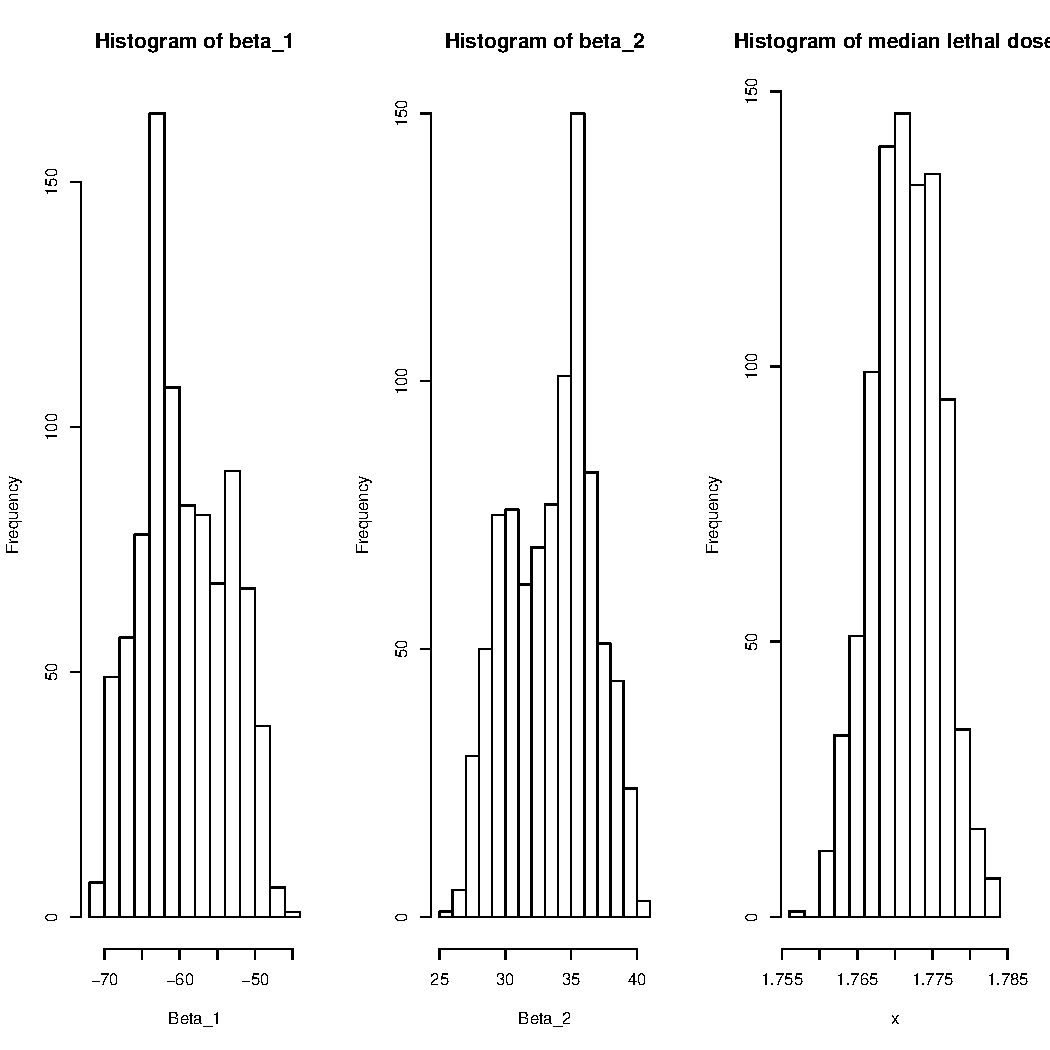
\includegraphics[width = \textwidth]{pic/HW3_2/b1.pdf}
        			\caption{Posterior distribution for $\bm{\beta}$ and $\mathrm{LD}_{50}$}
        		\end{subfigure}
        		\begin{subfigure}{0.45\linewidth}
        			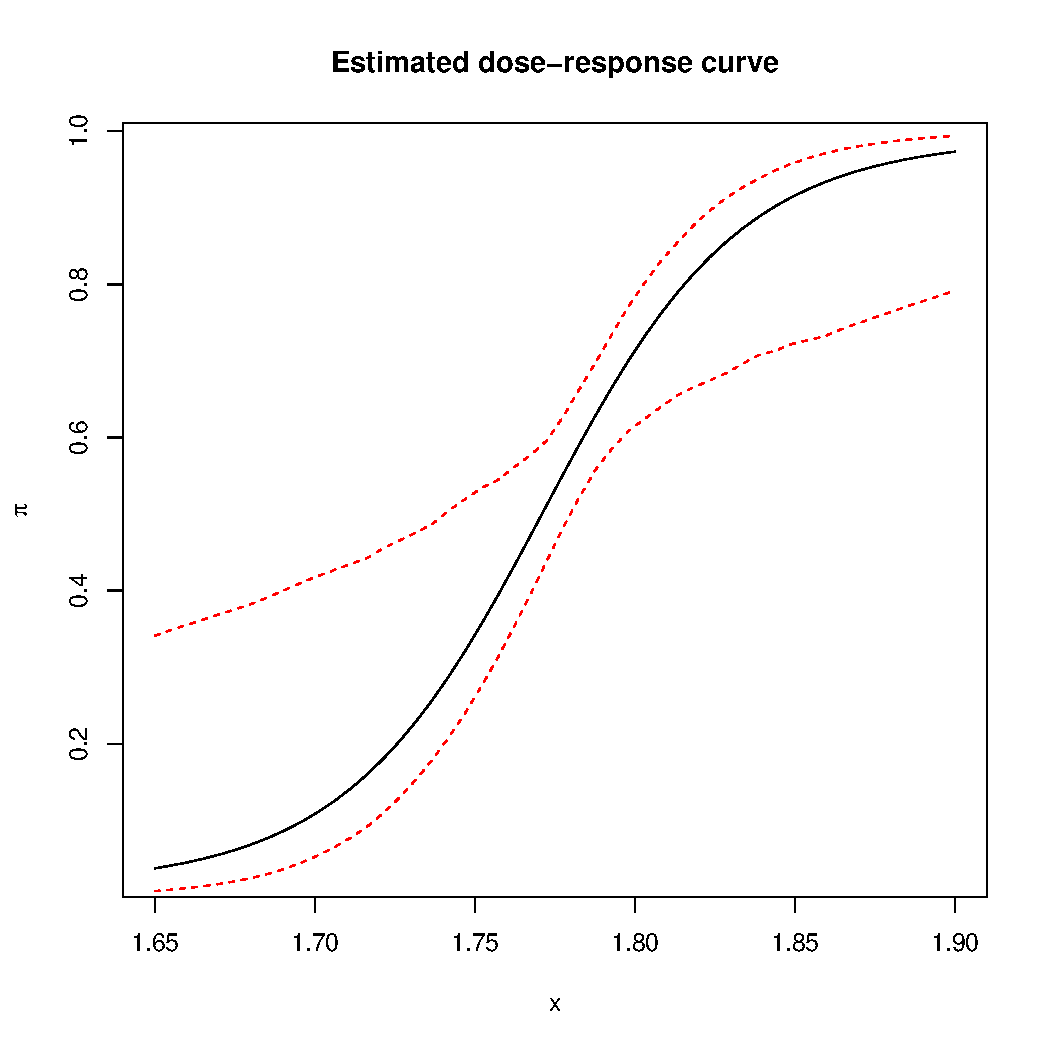
\includegraphics[width = \textwidth]{pic/HW3_2/b2.pdf}
        			\caption{Point and $95\%$ interval estimates for $\pi(x)$}
        		\end{subfigure}
        		\caption{Summary of model with logistic link function}
        		\label{8}
        	\end{figure}
        	\item[(c)]
        	Also, with Metropolis Hasting algorithm with 1000 samples and setting burn-in as $T = 100$, the posterior distributions for $\alpha, \beta_1, \beta_2$ and $\mathrm{LD}_50$ and point and centered $95\%$ interval estimates for the dose-response curve $\pi(x)$ are shown in Figure~\ref{9}.
        	\begin{figure}[ht!]
        		\centering
        		\begin{subfigure}{0.45\linewidth}
        			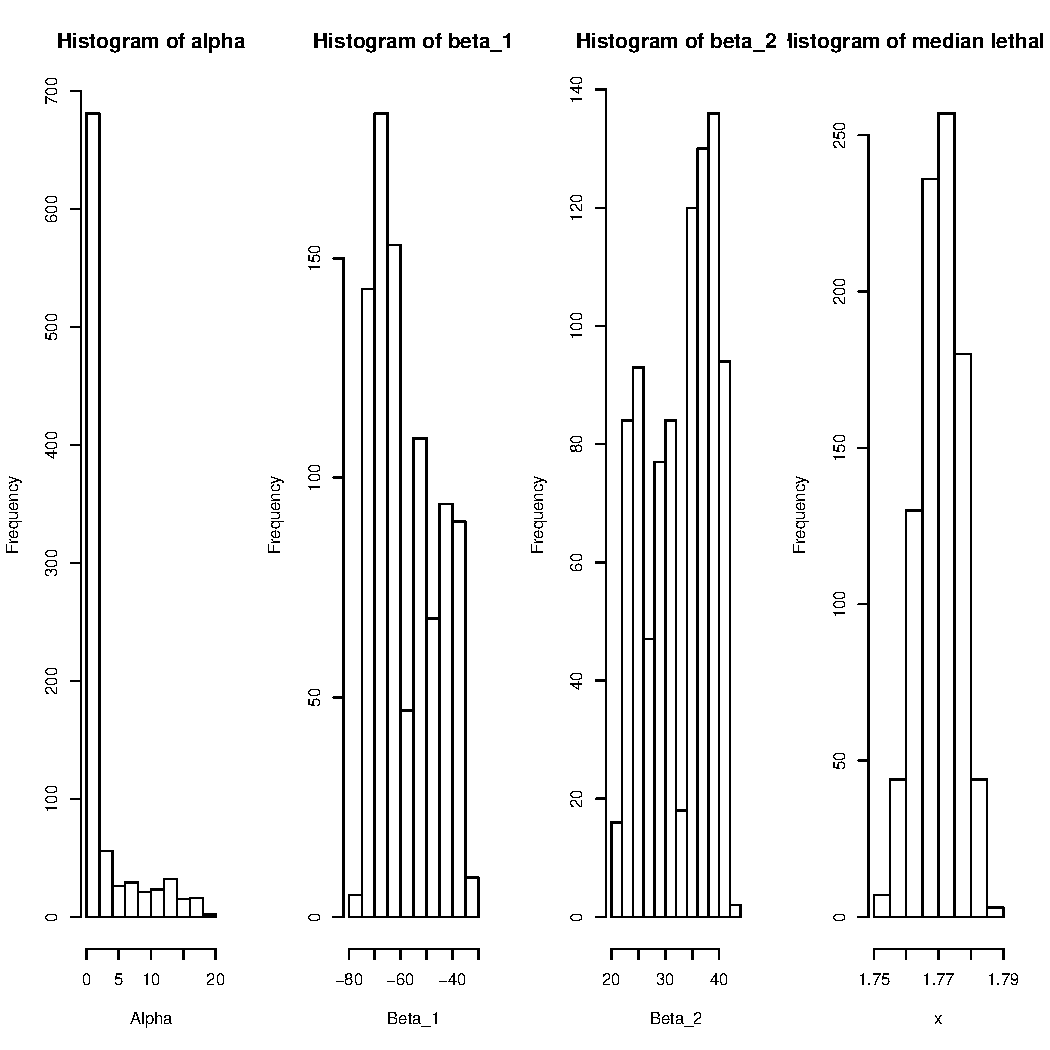
\includegraphics[width = \textwidth]{pic/HW3_2/c1.pdf}
        			\caption{Posterior distribution for $\alpha,\bm{\beta}$ and $\mathrm{LD}_{50}$}
        		\end{subfigure}
        		\begin{subfigure}{0.45\linewidth}
        			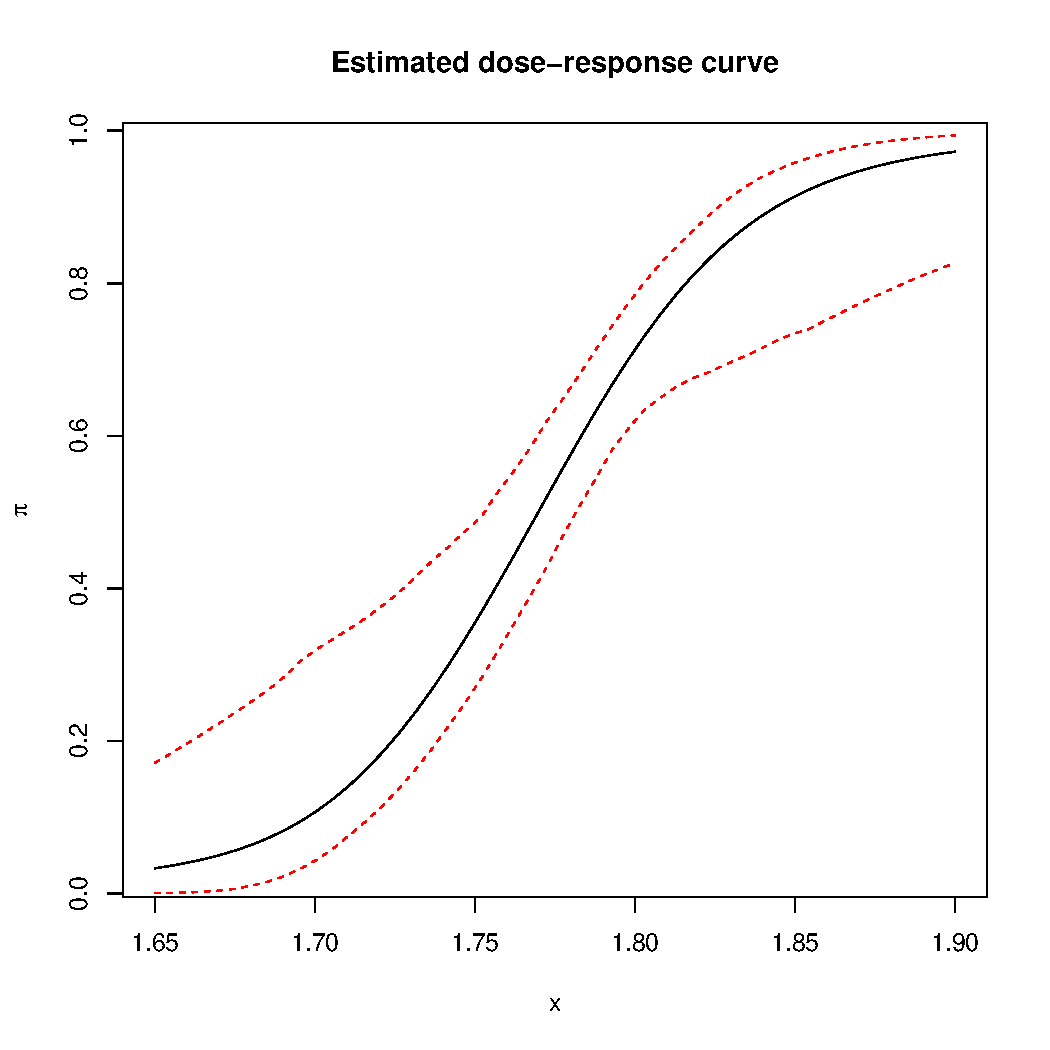
\includegraphics[width = \textwidth]{pic/HW3_2/c2.pdf}
        			\caption{Point and $95\%$ interval estimates for $\pi(x)$}
        		\end{subfigure}
        		\caption{Summary of model with general link function}
        		\label{9}
        	\end{figure}
        	\item[(d)]
        	From the estimated dose-response curves with respect to three models, the first and last models have narrower interval estimates than the second one which suggests that the second model has relative higher variance in interval estimation than other two models.\\
        	From the residual aspect, we check it by two aspects. First, for each $x_i$, we sample the posterior $\pi(x_i; \tilde{\bm{\beta}})$, where $\tilde{\bm{\beta}}$ follow the posterior distribution $Pr(\bm{\beta}| \bm y, \bm m, \bm x)$. And taking the mean of $\pi(x_i; \tilde{\bm{\beta}})$ as the estimated posterior predictive value denoted as $\hat{\pi}(x_i)$, Bayesian residual are estimated as $\hat{r}(x_i) = y_i/m_i-\hat{\pi}(x_i)$. The estimates for three model are in Table~\ref{10} Quadratic loss L measure is 
        	\begin{equation}
        	L_q(v) = \sum_{i = 1}^{n}var(\pi(x_i); \tilde{\beta}) + v \sum_{i = 1}^{n}(\hat{\pi}(x_1) - y_i/m_i)^2\,,
        	\end{equation}
        	where  $v = k/k+1$ is a tuning from $[0,1)$. For each model, we show the quadratic loss L measure $v = 0$ and $v \rightarrow 1$ in Table~\ref{10}, which suggests the first model has the smallest loss and so it performs better than others.
        	\begin{table}
        		\centering
        		\caption{The Bayesian residuals and quadratic loss L measure for three models}
        		\begin{tabular}{c|c|c|c|c|c|c|c|c|c|c}
        			\hline
        			x & 1.69 & 1.72 & 1.76 & 1.78 & 1.81 & 1.84 & 1.86 & 1.88 & $QL_0$ & $QL_1$\\
        			\hline
        			$res_1$ & -0.01 & 0.02 &-0.05& -0.04 &  0.07 & -0.01 & 0.01 & 0.01 & 0.022 &  0.032\\
        			\hline 
        			$res_2$ &  0.02 & 0.03 & -0.08& -0.10 & 0.04 & 0.01 & 0.04 & 0.03 & 0.029 & 0.053\\
        			\hline
        			$res_3$ & 0.02 & 0.01 & -0.11 & -0.12 & 0.05 & 0.03 & 0.06 & 0.04 & 0.024 & 0.060 \\
        			\hline
        		\end{tabular}
        		\label{10}
        	\end{table}
        	
        \end{itemize}
	
}
\end{enumerate}

\end{document}